% boston_20260828.tex
% Regional Special Sessions — Building Strong Health Systems for the Future
% Harvard T.H. Chan School of Public Health / Roche · Hilton Boston Back Bay
% Viernes 28 de agosto de 2026, 8:30–9:30 · Track América Latina
% Build instruction: 20260826_COMUNIDAD_BUILDINST_boston_deck_v1 (Debb)
% Compilar en Overleaf con pdfLaTeX. Subir junto con el .tex (misma carpeta):
%   wpp2024_lac_broad_age_groups.pdf  (gráfica oficial ONU, vectorial; alternativa: ...png)
% Restricción dura: cero ecuaciones, cero notación matemática, cero letras griegas.
% Cifras: solo las verificadas en verificaciones_boston_v1.md (17 verificaciones, 2026-08-26).

\documentclass[aspectratio=169,11pt]{beamer}

\usepackage[utf8]{inputenc}
\usepackage[T1]{fontenc}
\usepackage[spanish,es-noshorthands]{babel}
\usepackage[scaled=0.95]{helvet}
\usepackage{graphicx}
\usepackage{booktabs}
\usepackage{xcolor}

\usetheme{default}
\usecolortheme{default}
\usefonttheme{professionalfonts}

\setbeamertemplate{navigation symbols}{}
\setbeamertemplate{footline}[frame number]
\setbeamertemplate{itemize items}{--}
\setbeamertemplate{blocks}[default]

% Un solo color de acento, sobrio
\definecolor{acento}{RGB}{31,56,100}
\setbeamercolor{title}{fg=acento}
\setbeamercolor{frametitle}{fg=acento}
\setbeamercolor{structure}{fg=acento}
\setbeamercolor{itemize item}{fg=black}
\setbeamercolor{normal text}{fg=black,bg=white}
\setbeamercolor{footline}{fg=gray}
\setbeamerfont{frametitle}{size=\large,series=\bfseries}
\setbeamerfont{title}{size=\Large,series=\bfseries}
\setbeamerfont{footline}{size=\scriptsize}

% Utilería
\newcommand{\clave}[1]{\textcolor{acento}{\textbf{#1}}}
\newcommand{\destacar}[1]{\vspace{0.6em}\begin{center}\textbf{#1}\end{center}}
\newcommand{\pie}[1]{\vfill{\scriptsize\textcolor{gray}{#1}}}
\newcommand{\frase}[1]{\begin{center}\Large\textbf{#1}\end{center}}
\setlength{\leftmargini}{1.2em}

\title{Demografía, espacio fiscal y una nueva seguridad social}
\subtitle{Lo que esta semana no discutió}
\author{Héctor Juan Villarreal Páez}
\institute{ITED · Escuela de Gobierno y Transformación Pública · Tecnológico de Monterrey\\[0.4em]
Comunidad Latinoamericana del Conocimiento sobre Financiamiento de la Salud}
\date{Regional Special Sessions · \emph{Building Strong Health Systems for the Future}\\Boston, 28 de agosto de 2026}

\begin{document}

% =====================================================================
% APERTURA (2 min)
% =====================================================================

% ---------- 1. Portada ----------
\begin{frame}[plain]
  \titlepage
  % Logo solo en portada. Sustituir por el archivo institucional cuando esté disponible:
  % \begin{center}\includegraphics[height=1.1cm]{logo_tec.png}\end{center}
\end{frame}

% ---------- 2. Lo que esta semana no discutió ----------
\begin{frame}{Lo que esta semana no discutió}
  \begin{itemize}
    \item Cuatro días sobre compra estratégica, pago por valor, aseguramiento social y política de la reforma.
    \item Todo sobre \clave{cómo gastar mejor lo que hay}.
    \item Falta una pregunta: qué ocurre cuando cambia la estructura por edades.
  \end{itemize}
  \destacar{Dos restricciones: una ya está determinada; la otra se decide.}
\end{frame}

% =====================================================================
% MOVIMIENTO 1 — La demografía ya está decidida (10 min)
% =====================================================================

% ---------- 3. Gráfica UN WPP 2024 ----------
\begin{frame}{América Latina y el Caribe: población por grandes grupos de edad}
  \begin{center}
    % Gráfica oficial de Naciones Unidas (SVG del sitio WPP 2024, convertido a PDF vectorial).
    % Alternativa raster oficial con pie incrustado: {wpp2024_lac_broad_age_groups.png}
    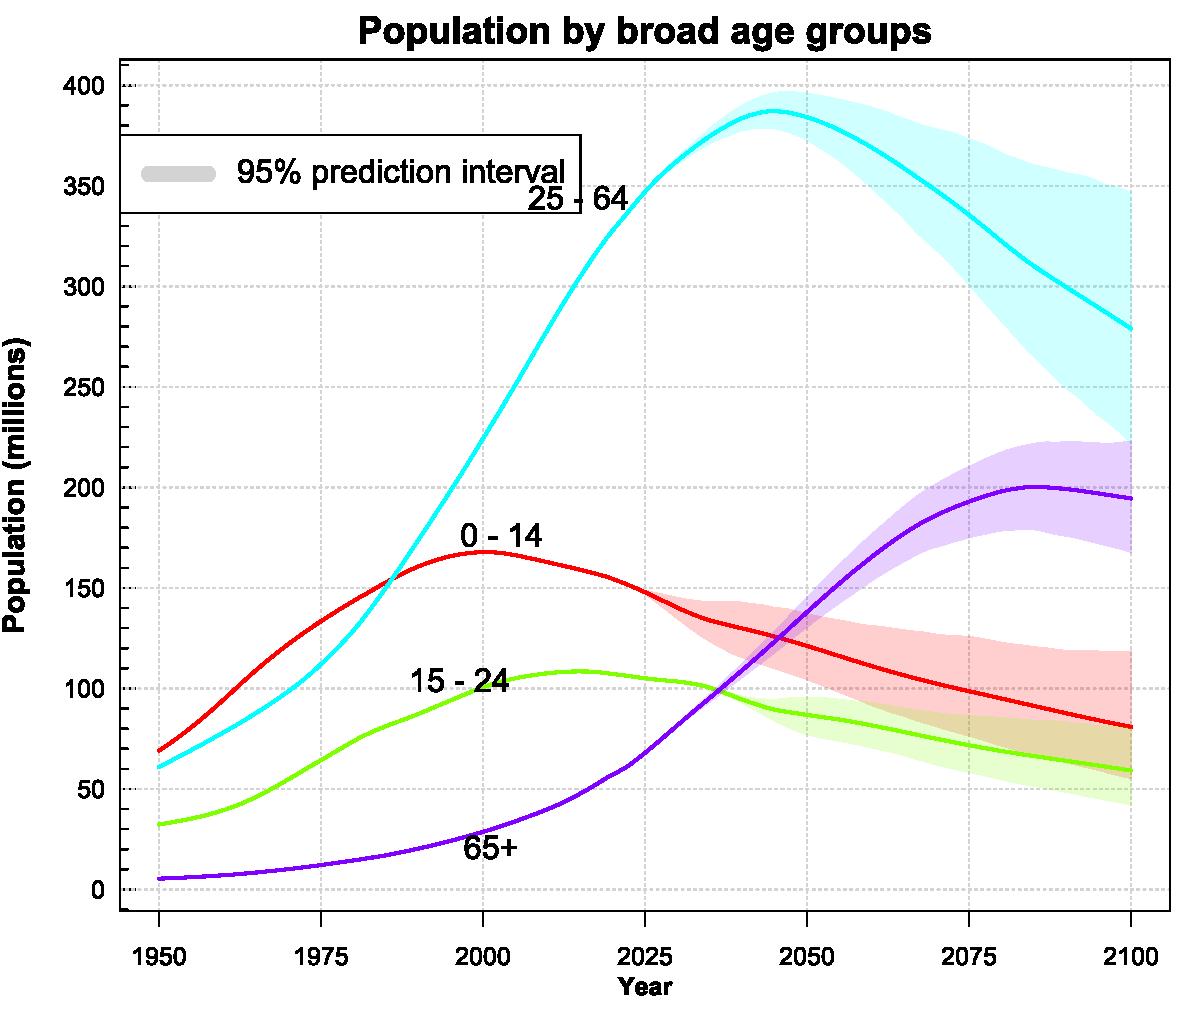
\includegraphics[height=0.78\textheight]{wpp2024_lac_broad_age_groups.pdf}\\[0.2em]
    {\scriptsize\textcolor{gray}{\copyright\ 2024 United Nations, DESA, Population Division. Licensed under Creative Commons license CC BY 3.0 IGO.
    United Nations, DESA, Population Division. \emph{World Population Prospects 2024}. http://population.un.org/wpp/}}
  \end{center}
\end{frame}

% ---------- 4. Lo que no es pronóstico ----------
\begin{frame}{Lo que no es pronóstico}
  \begin{itemize}
    \item La banda de 65 y más es casi imperceptible hasta mediados de la década de 2030; la de 25 a 64, hasta mediados de la de 2040.
    \item Son angostas porque \clave{esas personas ya nacieron}.
    \item Lo incierto es la fecundidad: la banda de 0 a 14 se abre desde el final de esta década.
    \item Hacia 2046 habrá más personas de 65 y más que niños de 0 a 14.
  \end{itemize}
  \destacar{El envejecimiento no es pronóstico. Es contabilidad.}
  \pie{Fuente: Naciones Unidas, DESA, División de Población, \emph{World Population Prospects 2024}, América Latina y el Caribe, variante media e intervalos de predicción al 95\,\% (amplitud menor al 5\,\% de la mediana hasta 2036 para 65 y más, y hasta 2046 para 25 a 64).}
\end{frame}

% ---------- 5. El envejecimiento del envejecimiento ----------
\begin{frame}{El envejecimiento del envejecimiento}
  \begin{itemize}
    \item Población de 80 años y más en la región: de \clave{12 millones en 2024 a 37 millones en 2050}.
    \item Su peso pasa de 1.9\,\% a 5.1\,\% de la población: se triplica en treinta años.
    \item Es el grupo donde manda la dependencia funcional y el cuidado de largo plazo.
  \end{itemize}
  \pie{Fuente: CEPAL (2025), \emph{Impactos económicos del envejecimiento en América Latina y el Caribe}, Serie Población y Desarrollo 140, p.~10, con base en Naciones Unidas (2024).}
\end{frame}

% ---------- 6. La ventana se cierra en 2028 ----------
\begin{frame}{La ventana se cierra en 2028}
  \begin{itemize}
    \item El bono demográfico regional concluye, en promedio, en \clave{2028}: dentro de dos años.
    \item Con grandes diferencias entre países: en Costa Rica, Colombia, Chile y Brasil ya terminó.
    \item De 65 millones de personas de 65 y más en 2024 a 138 millones en 2050.
  \end{itemize}
  \destacar{Lo que sigue ya no lo decide la demografía.}
  \pie{Fuente: CEPAL (2025), \emph{Impactos económicos del envejecimiento en América Latina y el Caribe}, Serie Población y Desarrollo 140, pp.~9--10, 33 y 46.}
\end{frame}

% =====================================================================
% MOVIMIENTO 2 — El espacio fiscal sí es una decisión (10 min)
% =====================================================================

% ---------- 7. El giro ----------
\begin{frame}[plain]
  \vfill
  \frase{Lo anterior está dado.\\[0.4em] Lo que sigue, no.}
  \vfill
\end{frame}

% ---------- 8. Gasto público críticamente bajo ----------
\begin{frame}{Gasto público críticamente bajo}
  \begin{itemize}
    \item México destina \clave{2.7\,\% del PIB} a salud desde el gobierno general, seguridad social incluida. El promedio regional es 4.1\,\%.
    \item El complemento no es ausencia de gasto: es gasto de bolsillo, no planeado, por urgencia.
    \item En México, \clave{41\,\%} del gasto corriente en salud sale del bolsillo de las familias. En la región, 30\,\%.
    \item Regresivo y empobrecedor.
  \end{itemize}
  \pie{Fuente: OMS, \emph{Global Health Expenditure Database}, 2023 (gasto en salud del gobierno general con fuentes domésticas, \% del PIB; gasto de bolsillo, \% del gasto corriente en salud). Promedio regional: agregado América Latina y el Caribe del Banco Mundial con la misma base.}
\end{frame}

% ---------- 9. Pensiones desplazan salud ----------
\begin{frame}{Pensiones desplazan salud}
  \begin{itemize}
    \item Las promesas previsionales maduraron antes de que se ampliara la base contributiva.
    \item Las pensiones no contributivas: avance real en cobertura, costo fiscal creciente.
    \item Sin reforma paramétrica, el gasto en pensiones desplaza todo lo demás.
  \end{itemize}
  \destacar{Reformar pensiones no es un tema separado de financiar salud: es su condición previa.}
\end{frame}

% ---------- 10. Un solo problema fiscal ----------
\begin{frame}{Un solo problema fiscal}
  \begin{itemize}
    \item Pensiones, salud y cuidados compiten por el \clave{mismo espacio presupuestario}.
    \item Se analizan como sistema, no como silos.
    \item Toda propuesta que dependa de impuestos generales debe demostrar que es financiable a veinte años.
  \end{itemize}
\end{frame}

% =====================================================================
% MOVIMIENTO 3 — La tenaza (10 min)
% =====================================================================

% ---------- 11. Dos cosas al mismo tiempo ----------
\begin{frame}{Dos cosas al mismo tiempo}
  \begin{itemize}
    \item Que la gente \clave{no se arruine} cuando se enferma.
    \item Que \clave{valga la pena} estar dentro del sistema contributivo.
    \item Casi todo lo que se ha intentado mejora una a costa de la otra.
  \end{itemize}
  \destacar{Esa es la tenaza.}
\end{frame}

% ---------- 12. La base no da ----------
\begin{frame}{La base no da}
  \begin{itemize}
    \item Informalidad estructural: \clave{cerca de la mitad del empleo} en la región; entre 22\,\% en Uruguay y 70\,\% en Ecuador.
    \item En México, Colombia, Paraguay, Ecuador y República Dominicana, menos de la mitad de los ocupados cotiza o está afiliado a pensiones. Costa Rica y Uruguay superan 70\,\%.
    \item Bismarck no falla por teoría. Falla por base contributiva estrecha.
  \end{itemize}
  \pie{Fuentes: OIT, \emph{Panorama Laboral 2025 de América Latina y el Caribe}, tasa de informalidad, primer semestre de 2025 (promedio de 12 países: 46.7\,\%); CEPALSTAT, ocupados que aportan o están afiliados a sistemas de pensiones, 2023--2024 (México 34\,\%, Colombia 43\,\%, Paraguay 25\,\%, Ecuador 35\,\%, República Dominicana 43\,\%, Costa Rica 73\,\%, Uruguay 77\,\%).}
\end{frame}

% ---------- 13. La trampa de la formalización ----------
\begin{frame}{La trampa de la formalización}
  \begin{itemize}
    \item El costo neto de ser formal: impuestos, contribuciones y pérdida de beneficios no contributivos. Para un asalariado, entre 20\,\% y 40\,\% del ingreso del hogar.
    \item Hallazgo central: el componente mayor \clave{no son los impuestos, son las contribuciones a seguridad social}. Impuestos y transferencias pesan poco; México es excepción parcial.
    \item Si el trabajador no valora lo que recibe, la contribución se percibe como impuesto puro.
  \end{itemize}
  \pie{Fuente: Fietz, Joubert, Ñopo, Ocampo, Packard, Posadas y Rodriguez Chamussy (2025), \emph{(In)Formalizing Jobs in Latin America and the Caribbean: Taxes, Benefits, and Labor Market Incentives}, Banco Mundial, cap.~5, pp.~90, 98 y 102 (seis países: Brasil, Colombia, El Salvador, México, Perú y Uruguay). Tasa de tributación a la formalización según Koettl y Weber (2012).}
\end{frame}

% ---------- 14. El escalón ----------
\begin{frame}{El escalón}
  \begin{itemize}
    \item Al formalizarse: un costo cierto e inmediato, y una pérdida posible de beneficios.
    \item Uruguay reconoció el desincentivo: desde 2022 \clave{suspendió el control del tope de ingreso} para las Asignaciones Familiares del Plan de Equidad, para promover el empleo formal; 21 mil hogares adicionales. Desde 2026 rige un tope alto.
    \item El dilema del paquete diferenciado: un paquete distinto para quien no cotiza crea un escalón; el mismo paquete elimina el incentivo a cotizar.
  \end{itemize}
  \pie{Fuentes: BPS, R.D.~39-5/2021 (suspensión desde el 1 de enero de 2022, prorrogada por R.D.~1-2/2023, 1-17/2024 y 26-1/2025) y R.D.~5-1/2026 (tope de 19.53 BPC per cápita para 2026); MEF, \emph{Rendición de Cuentas 2023, Exposición de Motivos}, p.~81; Fietz et al. (2025), pp.~133--136; Bergolo y Cruces (2021), \emph{Journal of Public Economics} 193.}
\end{frame}

% =====================================================================
% MOVIMIENTO 4 — Qué ha intentado la región (5 min)
% =====================================================================

% ---------- 15. Cinco casos, cinco piezas ----------
\begin{frame}{Cinco casos, cinco piezas}
  \begin{center}\small
  \begin{tabular}{@{}p{2.0cm}p{5.6cm}p{5.6cm}@{}}
    \toprule
    \textbf{País} & \textbf{Qué resolvió} & \textbf{Qué le sigue faltando} \\
    \midrule
    Costa Rica & Seguro único de la CCSS: 90\,\% de la población asegurada & Sostenerlo con fecundidad de 1.12 y un cuarto de mayores en 2050 \\[0.3em]
    Uruguay    & Seguro Nacional de Salud: tres cuartos del país dentro del FONASA & El cuarto que sigue fuera del seguro nacional \\[0.3em]
    Colombia   & Afiliación de 98\,\%; plan de beneficios unificado desde 2012 & Informalidad de 54\,\%: el régimen subsidiado ya supera al contributivo \\[0.3em]
    México     & Un prestador federal único para quien no tiene seguridad social & Estabilidad: tres arquitecturas entre 2019 y 2023 \\[0.3em]
    Brasil     & SUS universal desde 1988: un solo sistema público & Un cuarto con plan privado, deducible del impuesto sobre la renta sin tope \\
    \bottomrule
  \end{tabular}
  \end{center}
  \destacar{Elegir Beveridge no evita la dualidad; solo cambia el lugar por donde aparece.}
  \pie{Fuentes: INEC Costa Rica, ENAHO 2024 y comunicado de fecundidad 2024; ONU DESA, WPP 2024; Presidencia de Uruguay (dic.\ 2025) e INE, Censo 2023; MinSalud Colombia, cifras de afiliación julio 2026, y DANE, abril--junio 2026; Diario Oficial de la Federación, 29-XI-2019, 31-VIII-2022 y 29-V-2023; ANS, junio 2026, y Lei 9.250/1995, art.~8.}
\end{frame}

% =====================================================================
% MOVIMIENTO 5 — Una nueva seguridad social (6 min)
% =====================================================================

% ---------- 16. Ampliar, no abandonar ----------
\begin{frame}{Ampliar, no abandonar}
  \begin{itemize}
    \item Quien puede contribuir, \clave{contribuye}.
    \item Quien no cotiza paga al menos un tramo de su prima, proporcional a su ingreso.
    \item El gobierno cubre la prima completa solo para los más necesitados.
  \end{itemize}
  \destacar{Lógica contributiva ampliada, no abandonada.}
\end{frame}

% ---------- 17. Dos instrumentos ----------
\begin{frame}{Dos instrumentos}
  \begin{itemize}
    \item \clave{Cuotas contributivas rediseñadas}: canalizadas a salud, con vínculo claro entre contribución y beneficio. Que el trabajador perciba valor, no impuesto.
    \item \clave{Primas graduadas para no cotizantes}: copago proporcional al ingreso; prima completa a cargo del Estado solo para los más vulnerables.
  \end{itemize}
  \destacar{Todos dentro del sistema de seguros. Nadie afuera en un esquema paralelo.}
\end{frame}

% ---------- 18. Consolidar transferencias ----------
\begin{frame}{Consolidar transferencias}
  \begin{itemize}
    \item Programas fragmentados con umbrales rígidos: al cruzarlos, pérdida abrupta.
    \item Un \clave{impuesto negativo sobre la renta} como puente: el beneficio decrece suavemente, no hay salto, el trabajador siempre gana al formalizarse.
    \item Condición necesaria: observar ingresos. Hoy factible por digitalización de pagos y facturación electrónica.
  \end{itemize}
\end{frame}

% ---------- 19. El guiño ----------
\begin{frame}[plain]
  \vfill
  \frase{Hay un tercer instrumento posible: prefondear el gasto de salud de la vejez.\\[0.6em]
  \normalsize\normalfont Sobre él hay una pregunta, no una recomendación. Volvemos al cierre.}
  \vfill
\end{frame}

% =====================================================================
% MOVIMIENTO 6 — La doble prueba (2 min)
% =====================================================================

% ---------- 20. Dos preguntas para todo ----------
\begin{frame}{Dos preguntas para todo}
  \begin{enumerate}
    \item ¿Es financiable a lo largo de la transición demográfica, sin dinámicas de deuda insostenibles?
    \item ¿Fortalece o debilita el incentivo del trabajador a cotizar?
  \end{enumerate}
  \destacar{Fallar en cualquiera de las dos es debilidad estructural.}
\end{frame}

% =====================================================================
% PARTE II — La Comunidad (15 min)
% =====================================================================

% ---------- 21. El hueco ----------
\begin{frame}{El hueco}
  \begin{itemize}
    \item La región discute la \clave{cobertura} de sus sistemas de salud con seriedad desde hace décadas.
    \item Discute mucho menos su \clave{solvencia de largo plazo}.
    \item Con qué recursos, durante cuánto tiempo y a costa de qué otras obligaciones públicas.
  \end{itemize}
\end{frame}

% ---------- 22. Qué es y quiénes ----------
\begin{frame}{Comunidad Latinoamericana del Conocimiento sobre Financiamiento de la Salud}
  \small
  \begin{itemize}
    \item Núcleo fundador: Tecnológico de Monterrey (coordinación, Héctor Villarreal); Universidad de los Andes (Ramiro Guerrero); Pontificia Universidad Católica de Chile (Pablo Celhay). Horizonte de cinco años; vocación de red regional.
    \item Financiamiento semilla de Roche al Tecnológico de Monterrey, declarado abiertamente.
    \item Cuatro reglas de independencia: sin veto ni revisión previa vinculante; declaración de todo financiamiento; rechazo documentado de cualquier condicionamiento; y
  \end{itemize}
  \destacar{La producción puede analizar críticamente el gasto farmacéutico y los precios de los medicamentos, sin excepción por identidad del patrocinador.}
\end{frame}

% ---------- 23. Cuatro preguntas abiertas ----------
\begin{frame}{Cuatro preguntas abiertas}
  \begin{enumerate}
    \item Cuánto pesa el financiamiento privado, y qué parte del gasto catastrófico de bolsillo puede convertirse en prepago mancomunado.
    \item Bajo qué reglas un instrumento privado complementa el pool público en vez de vaciarlo.
    \item Si detectar antes ahorra recursos al sistema, o adelanta y prolonga el gasto.
    \item Si las promesas de pensiones dejan margen para financiar salud a veinte años.
  \end{enumerate}
\end{frame}

% ---------- 24. El pedido y la cita ----------
\begin{frame}{El pedido y la cita}
  \begin{itemize}
    \item Un \clave{mapa regional de investigadores} en financiamiento de la salud.
    \item Acceso a datos, donde exista la posibilidad.
    \item Reunión de trabajo: \clave{San José, Costa Rica, 5 al 7 de octubre de 2026}.
  \end{itemize}
\end{frame}

% ---------- 25. Cierre ----------
\begin{frame}[plain]
  \vfill
  \frase{¿Podemos diseñar sistemas de protección social que la gente valore lo suficiente como para querer participar, y que los gobiernos puedan financiar a lo largo de la transición demográfica?}
  \vfill
  \begin{center}\small
    Héctor Juan Villarreal Páez · hjvp@itesm.mx\\
    Escuela de Gobierno y Transformación Pública · Tecnológico de Monterrey\\
    Karina Sánchez · karina.sanchezbazan@tec.mx
  \end{center}
  \vfill
\end{frame}

\end{document}
